\documentclass[12pt, a5paper, french]{memoir}
\usepackage{geometry}
\usepackage[utf8]{inputenc}
\usepackage[T1]{fontenc}
\usepackage{fourier}
\usepackage{microtype}
\usepackage{dramatist}
\usepackage{lineno}
\usepackage{hyperref}
\usepackage{graphicx}
\usepackage{babel}

\renewcommand{\scenename}{Scène}
\renewcommand{\casttitlename}{Personnages}
\setlength{\beforesceneskip}{2em}%
\renewcommand{\printscenenum}{\scenenumfont \thescene{} --}
\renewcommand{\speakslabel}[1]{\textsc{#1}. ---}
\setlength\linenumbersep{20pt}

\makepagestyle{myps}
\makeevenfoot{myps}{\thepage}{}{}
\makeoddfoot{myps}{}{}{\thepage}

\title{L'anneau de Gygès}
\author{Libre Édu\thanks{Texte sous licence \href{http://creativecommons.org/licenses/by-sa/4.0/deed.fr}{CC BY-SA}, inspiré d’une fable racontée dans la \textit{République} de Platon.}}

\Character[Gygès]{Gygès}{Gyges}
\Character[Candaule, le roi]{Candaule}{Candaule}
\Character[Nyssia, la fiancée du roi]{Nyssia}{Nyssia}
\Character[Laurel, le serviteur du roi]{Laurel}{Laurel}
\Character[Hardy, le serviteur de Nyssia]{Hardy}{Hardy}
\Character[Bonnie, une voleuse]{Bonnie}{Bonnie}
\Character[Clyde, un voleur]{Clyde}{Clyde}
\Character[Leonardo, un berger]{Leonardo}{Leonardo}
\Character[Donatello, un berger]{Donatello}{Donatello}
\Character[Michelangelo, un berger]{Michelangelo}{Michelangelo}
\Character[Raffaello, un berger]{Raffaello}{Raffaello}
\Character[Tiziano, un berger]{Tiziano}{Tiziano}


\begin{document}

\maketitle
\thispagestyle{empty}
\vfill
\begin{figure}[h]
\centering
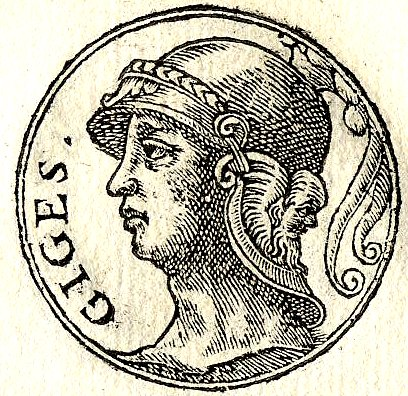
\includegraphics[scale=1]{Gyges.jpg}
\end{figure}
\vfill

\newpage
\renewcommand\contentsname{Sommaire}
\tableofcontents*
\thispagestyle{empty}

\DramPer*
\thispagestyle{empty}

\newpage
\pagestyle{myps}
\begin{linenumbers}


\scene[Gygès]
\StageDir{\Gyges, \Bonnie, \Clyde}
\begin{drama}
\Bonniespeaks Connais-tu la dernière nouvelle ?
\Clydespeaks Quelle nouvelle ?
\Bonniespeaks Le roi vient de s’acheter la dernière Nintendo, la 3DS~XXL.
\Clydespeaks Comment sais-tu ça ?
\Bonniespeaks C’est écrit dans le journal. Si seulement tu savais lire\dots
\Clydespeaks Pff ! Le journal, il suffit de le regarder à la télé !
\Bonniespeaks Au lieu de dire des bêtises, dis-moi plutôt comment on va faire pour voler cette console.
\Clydespeaks Mais\dots{} c’est qui là-bas ?
\Bonniespeaks C’est Gygès, au pied de son arbre, en train de surveiller ses chèvres.
\Clydespeaks Allons le saluer. \direct{À Gygès.} Gygès, tu viens avec nous ? On va faire un plan pour voler la dernière console du roi.
\Gygesspeaks Moi, Monsieur, je suis honnête, je ne vole pas, je respecte les lois.
\newpage
\Bonniespeaks Gygès, au lieu de faire le malin, réponds plutôt à la question suivante. Tu ne voles pas, car tu as peur de te faire arrêter, ou parce que tu penses que c’est bien de respecter la loi ? Si tu avais de super-pouvoirs et que tu es sûr de ne pas te faire attraper, que ferais-tu ? Respecterais-tu la loi, ou pas ?

\scene[L’anneau]
\StageDir{\Gyges}
\Gygesspeaks Tiens, une crevasse ? Je ne l’avais jamais remarquée. On dirait qu’il y a quelque chose au fond. Une boite ? Il y a un texte écrit dessus : \og Ô mortel, n’envie jamais le bonheur d’un autre homme. \fg{} \direct{Ouvre la boite.} Tiens, un anneau ! \direct{Passe l’anneau à son doigt, le chaton à l’extérieur.} Bon, rien ne se passe ! Ce n’est pas tout, mais il faut que je retourne au village, il y a le conseil des bergers.
\newpage

\scene[La mission]
\StageDir{\Gyges, \Leonardo, \Donatello, \Michelangelo, \Raffaello, \Tiziano}
\Leonardospeaks Gygès, dépêche-toi, on n’a pas que ça à faire. J’ai des pommes de terre à éplucher.
\Donatellospeaks Oh ! On est ici pour parler de chèvres, pas de patates !
\Michelangelospeaks Bon. Qui va voir le roi pour faire un rapport sur l'état des troupeaux ?
\Raffaellospeaks Pas moi.
\Tizianospeaks Moi.
\Donatellospeaks Non, pas toi. La dernière fois, tu as eu un problème avec le roi.
\Leonardospeaks Bon, alors c’est Gygès qui va aller voir le roi.
\Gygesspeaks \direct{À lui-même.} Je vais tourner le chaton de ma bague vers l’intérieur, voir ce que se passe.
\Leonardospeaks Il est où Gygès ? Saperlipopette, il a encore disparu.
\Raffaellospeaks C’est vrai, ça. Il était encore là, il y a 5~secondes.
\newpage
\Gygesspeaks \direct{Tournant le chaton vers l’extérieur.} C’est moi que vous cherchez ?
\Tizianospeaks Ah, enfin, te voilà de retour! Bon, nous avons décidé que c’est toi qui iras voir le roi.
\Gygesspeaks D’accord. Je m’en vais de ce pas le voir.

\scene[La fiancée]
\StageDir{\Gyges, \Candaule, \Nyssia, \Laurel}
\Laurelspeaks Votre Majesté, Gygès vient d’arriver.
\Candaulespeaks Bien, faites-le entrer.
\Gygesspeaks Votre Majesté.
\Candaulespeaks Gygès, mon ami, comment vont les affaires ?
\Gygesspeaks Bien.
\Candaulespeaks Avant de parler affaires, il faut que je te présente ma fiancée. Passe un peu de temps avec elle et dis-moi ce que tu en penses.
\Gygesspeaks Votre Majesté, cela ne se fait pas\dots
\Candaulespeaks J’insiste. \direct{À Nyssia.} Nyssia, viens voir ici. Je dois partir, j’ai des affaires à régler. Je te présente Gygès, un ami, qui va te tenir compagnie pour le diner.
\newpage

\scene[L’assassinat]
\StageDir{\Gyges, \Nyssia, \Hardy}
\Gygesspeaks \direct{À lui-même.} J’ai bien mangé. Il en a de la chance le roi, d’épouser une si belle dame. Je l’envie.
\Hardyspeaks Madame, je viens d’apprendre que le roi est furieux de la conduite de Gygès. Il veut le tuer.
\Nyssiaspeaks Vite, va le prévenir Gygès du sort qui l’attend.
\Hardyspeaks Monsieur, vous courez un grand danger, le roi veut votre mort.
\Gygesspeaks Ha ! Le scélérat ! Je vais utiliser mon anneau d’invisibilité pour le tuer pendant son sommeil.
\newpage

\scene[La question]
\StageDir{\Bonnie, \Clyde}
\Bonniespeaks Connais-tu la dernière nouvelle ?
\Clydespeaks Quelqu’un a volé la console du roi ?
\Bonniespeaks Non ! Le roi a été assassiné. Maintenant, c’est Gygès qui est roi à la place du roi.
\Clydespeaks Le roi est mort, vive le roi !
\Bonniespeaks Mais cela ne répond pas à la question.
\Clydespeaks Quelle question ?
\Bonniespeaks Imagine que, lorsque tu fais une très grosse bêtise, tu sais d’avance qu’on ne pourra jamais savoir que c’est toi qui a fait la bêtise. Que ferais-tu ? Bêtise, ou pas bêtise ? Faire ou ne pas faire, telle est la question.

\end{drama}
\end{linenumbers}

\centering
\vfill
\textsc{Fin}
\vfill
\thispagestyle{empty}

\end{document}